\section{Nonlinear Least Squares}
\subsection{Theory}
Nonlinear Least Squares solves a nonlinear, overconstrained system of equations by minimizing the squared residuals of each observation equation.  A Taylor Series expansion is utilized to linearize the equation and iteratively calculate the gradient of the function to determine a local minima.  Optionally, a weight matrix($W$) may be used.  Remove the W term, or replace with an identity matrix if a Weight matrix is not desired.  Covariances may be 0s if not known.

*Note that if the scale of the variance-covariance in the weight matrix is known to be 1, then the computed reference variance should be inspected to ensure it passes the $\chi^2$ goodness of fit test.  If it passes the test, the Covariance matrix should NOT be multiplied by the reference variance.  See definition of reference variance for the reasoning.

\subsection{Assumptions}
\begin{itemize}
	\item No Outliers/Blunders. Nonlinear Least Squares is not robust to outliers (consider RANSAC/Robust Weighting if outliers)
	\item System of equations is nonlinear (eg. derivative wrt at least one unknown is a function of one of the other unknowns)
	\item System is over-constrained (eg. Number of Observation Equations > Number of Unknowns)
	\item Error only in dependent variable (eg. mx+b = y + v $\rightarrow$ error only in y dimension)
	\item $X_0$ must be a reasonable guess, otherwise the solution might settle on an incorrect local minima, rather than the global minimum.	
\end{itemize}
\subsection{Equations}
\[
AX = L + V
\]
\[
WJ\Delta X=WK+WV 
\]
\[
m = \text{number of observations} \hspace{1cm} 
n = \text{number of unknowns}
\]
\[
dof = \text{degrees of freedom (\# of redundant observations)} = m-n
\]
\[
i = \text{loop iteration}
\]
\[
\text{Observation Equations =  } F_m(x_1,x_2,...,x_n) = l_m \text{ (note: }AX\text{ is obs eqn, L is }[l_1,l_2...,l_m] \text{ )}
\]
\[
J_i = \begin{bmatrix}
\ddx{F_1}{x_1} & \ddx{F_1}{x_2} & \dots & \ddx{F_1}{x_n} \\
\ddx{F_2}{x_1} & \ddx{F_2}{x_2} & \dots & \ddx{F_2}{x_n} \\
\vdots & \vdots & \ddots& \vdots \\
\ddx{F_m}{x_1} & \ddx{F_m}{x_2} & \dots & \ddx{F_m}{x_n} \\
\end{bmatrix}
\hspace{0.5cm}
\Delta X = 
\begin{bmatrix}
\Delta x_1 \\ \Delta x_2 \\ \vdots \\ \Delta x_n
\end{bmatrix}
\hspace{0.5cm}
K_i = 
\begin{bmatrix}
l_1 - F_1(\hat{X_i}) \\ l_2 - F_2(\hat{X_i})\\ \vdots \\ l_m - F_m(\hat{X_i})
\end{bmatrix}
\hspace{0.5cm}
V = 
\begin{bmatrix}
v_1 \\ v_2 \\ \vdots \\ v_m
\end{bmatrix}
\]
\[
W = 
\begin{bmatrix}
\sigma_{11}^2 & \sigma_{12}^2 & \dots & \sigma_{1m}^2 \\ 
\sigma_{21}^2 & \sigma_{22}^2 & \dots & \sigma_{2m}^2 \\ 
\vdots & \vdots & \ddots& \vdots \\
\sigma_{m1}^2 & \sigma_{m2}^2 & \dots & \sigma_{mm}^2 \\ 
\end{bmatrix}
^{-1}
\hspace{1cm}
\text{Initial Guess } \hat{X_0} = 
\begin{bmatrix}
x_1 \\ x_2 \\ \vdots \\ x_n
\end{bmatrix}
\]
\subsubsection{Loop Equations:}
Loop until $\Delta X $ is small, or more robustly, loop until $S_0^2$ increases.  $S_0^2$ will increase slightly when you get down to really really small numbers and the cpu starts rounding.  Caveat: it will also increase if you have a really bad initial guess, and it starts diverging.
\vspace{0.15cm}
\begin{align*}
\text{Recalculate } K_i & = K(\hat{X_i})\\
\text{Recalculate } J_i & = J(\hat{X_i})\\
\text{Loop Delta Estimate = }\Delta X &= inv(J_i^TWJ_i)J_i^TWK_i \\
\text{Loop Estimate = } \hat{X}_i &= X_{i-1}+\Delta X \\
\text{Residuals} = V &= J_i\Delta \hat{X_i} - K_i \\
\text{Reference Variance} = S_0^2 &= \dfrac{V^TWV}{dof}
\end{align*}
	
\subsubsection{Final Calculations}
\begin{align*}
	\text{Unknowns} &= \hat{X} = \hat{X}_i \text{   (Final Loop Estimate)}\\
	\text{Cofactor Matrix} &= Q_{xx} = inv(J^TWJ) \\
	\text{Covariance Matrix of Unkowns} &= \Sigma_{xx} = S_0^2 \times Q_{xx} \\
	\text{Covariance Matrix of Observations} &= \Sigma_{\hat{l}\hat{l}} = J \Sigma_{xx} J^T \\
	\text{Standard Deviation of Solved Unknowns} &= \sigma_{\hat{X}} = \sqrt{diag(\Sigma_{xx})} \\
	\text{Predicted L} &= \hat{L} = AX \\
	\text{R$^2$ (model skill)} &= \text{Not valid for nonlinear least squares} \\
	\text{RMSE } &= \sqrt{\dfrac{VV^T}{m}} \\
\end{align*}
\clearpage
\subsection{Sample Problem}

Given a timeseries dataset (ts.csv) of a harmonic signal with a known period and estimated variance for each measurement, calculate the amplitude and Phase.
\begin{figure}[H]
	\centering
	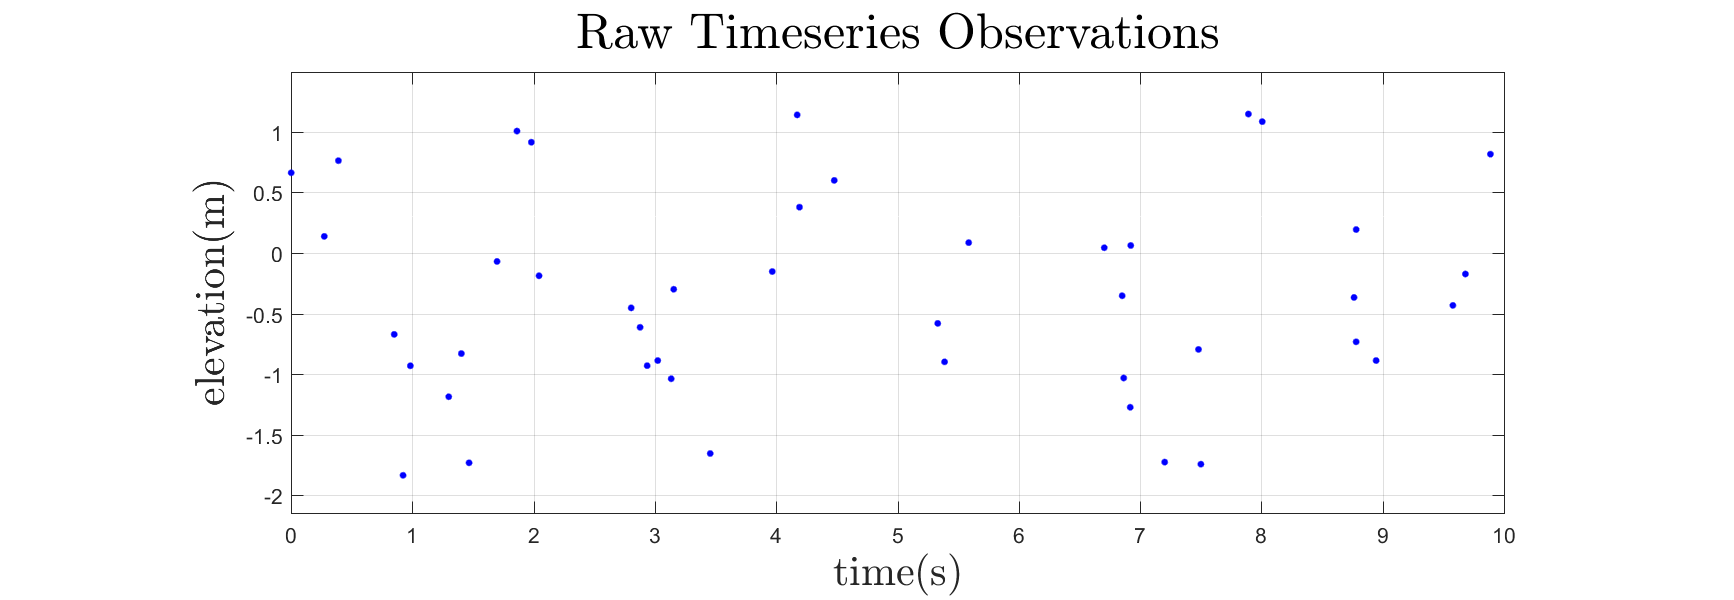
\includegraphics[height = 2in]{nonlineardata.png}
\end{figure}

The governing equation for the system is:
\[
F:\hspace{1cm} A \times \sin(\dfrac{2\pi}{T}t + \phi) = y
\]

Where:

\begin{align*}
\text{Amplitude(m)} &= A \\
\text{Period(s)}    &= T = 2 \\
\text{Phase(s)}     &= \phi \\
\text{Elevation Measurement(m)} &= y \\
\text{Time Measurement(s)} &= t \\	
\end{align*}

Note that this system is Nonlinear due to the Phase term.  The Jacobian is solved using the partial derivatives.

\[
J_i = \begin{bmatrix}
	\ddx{F_1}{A} &  \ddx{F_1}{\phi} \\
	\ddx{F_2}{A} & \ddx{F_2}{\phi} \\
	\vdots & \vdots \\
	\ddx{F_m}{A} & \ddx{F_m}{\phi} \\
\end{bmatrix}
=
\begin{bmatrix}
\sin(\dfrac{2\pi}{T}t_1 + \phi_i) & A_i \times \cos(\dfrac{2\pi}{T}t_1 + \phi_i) \\
\sin(\dfrac{2\pi}{T}t_2 + \phi_i) & A_i \times \cos(\dfrac{2\pi}{T}t_2 + \phi_i) \\
\vdots & \vdots \\
\sin(\dfrac{2\pi}{T}t_m + \phi_i) & A_i \times \cos(\dfrac{2\pi}{T}t_m + \phi_i) \\
\end{bmatrix}
\]
\[
\Delta X = 
\begin{bmatrix}
\Delta A \\ \Delta \phi
\end{bmatrix}
\hspace{1cm}
K_i = 
\begin{bmatrix}
l_1 - F_1(\hat{X_i}) \\ l_2 - F_2(\hat{X_i})\\ \vdots \\ l_m - F_m(\hat{X_i})
\end{bmatrix}
=
\begin{bmatrix}
y_1 - A_i \times \sin(\dfrac{2\pi}{T}t_1 + \phi_i) \\
y_2 - A_i \times \sin(\dfrac{2\pi}{T}t_2 + \phi_i) \\
\vdots \\
y_m - A_i \times \sin(\dfrac{2\pi}{T}t_3 + \phi_i)
\end{bmatrix}
\]
\[
\text{Initial guess from looking at the plot } = X_0 = 
\begin{bmatrix}
A_0 \\ \phi_0
\end{bmatrix}
=
\begin{bmatrix}
1.5 \\ 1
\end{bmatrix}
\]
\clearpage
Solving using Equations:
\begin{table}[H]
\centering
\begin{tabular}{|c|c|c|}
\toprule
$n = 2$& %NEWCOLUMN
$m = 50$& %NEWCOLUMN
$dof = 48$\\ %NEWROW
\midrule
$\hat{X} = $$
 \begin{bmatrix}
1.43\\
0.90\\
\end{bmatrix}
$
& %NEWCOLUMN
$S_0^2 = 2.77$ & %NEWCOLUMN
$Q_{xx} = $ $
 \begin{bmatrix}
0.01&0.00\\
0.00&0.00\\
\end{bmatrix}
$
\\ %NEWROW
\midrule
$\Sigma_{xx} = $ $
 \begin{bmatrix}
0.0202&0.0004\\
0.0004&0.0003\\
\end{bmatrix}
$
& %NEWCOLUMN
$\sigma_{\hat{X}} = $ $
 \begin{bmatrix}
0.1421\\
0.0174\\
\end{bmatrix}
$
& %NEWCOLUMN
$RMSE = 0.66$\\ %NEWROW
\bottomrule
\end{tabular}
\end{table}


A two tailed $\chi^2$ Goodness of Fit Test is performed at the 0.05 Significance level:
\begin{align*}
\text{Null Hypothesis } H_0 &: S_0^2 = 1 \\
\text{Alternative Hypothesis } H_a &: S_0^2 \neq 1 \\
\text{Significance } &: \alpha = 0.05 
\end{align*}
Test Statistic:
\[
\chi^2 = \dfrac{vS_0^2}{\sigma^2} = \dfrac{dof\times S_0^2}{1} = dof\times S_0^2 = 44.95
\]
Rejection Region:
\begin{align*}
44.95 = \chi^2 &> \chi_{(\alpha/2,dof)}^2 = 30.75 \hspace{1cm} &(PASS)\\
44.95 = \chi^2 &< \chi_{(1-\alpha/2,dof)}^2 = 69.02 \hspace{1cm} &(PASS)
\end{align*}
Results:

The results pass the $\chi^2$ Goodness of Fit Test at the 0.05 significance level, so redo the final calculations with $S_0^2$ equal to 1.


\begin{table}[H]
\centering
\begin{tabular}{|c|c|c|}
\toprule
$S_0^2 = 1.00$ & %NEWCOLUMN
$\Sigma_{xx} = $ $
 \begin{bmatrix}
0.0196&-0.0010\\
-0.0010&0.0027\\
\end{bmatrix}
$
& %NEWCOLUMN
$\sigma_{\hat{X}} = $ $
 \begin{bmatrix}
0.1399\\
0.0515\\
\end{bmatrix}
$
\\ %NEWROW
\bottomrule
\end{tabular}
\end{table}

\begin{figure}[H]
	\centering
	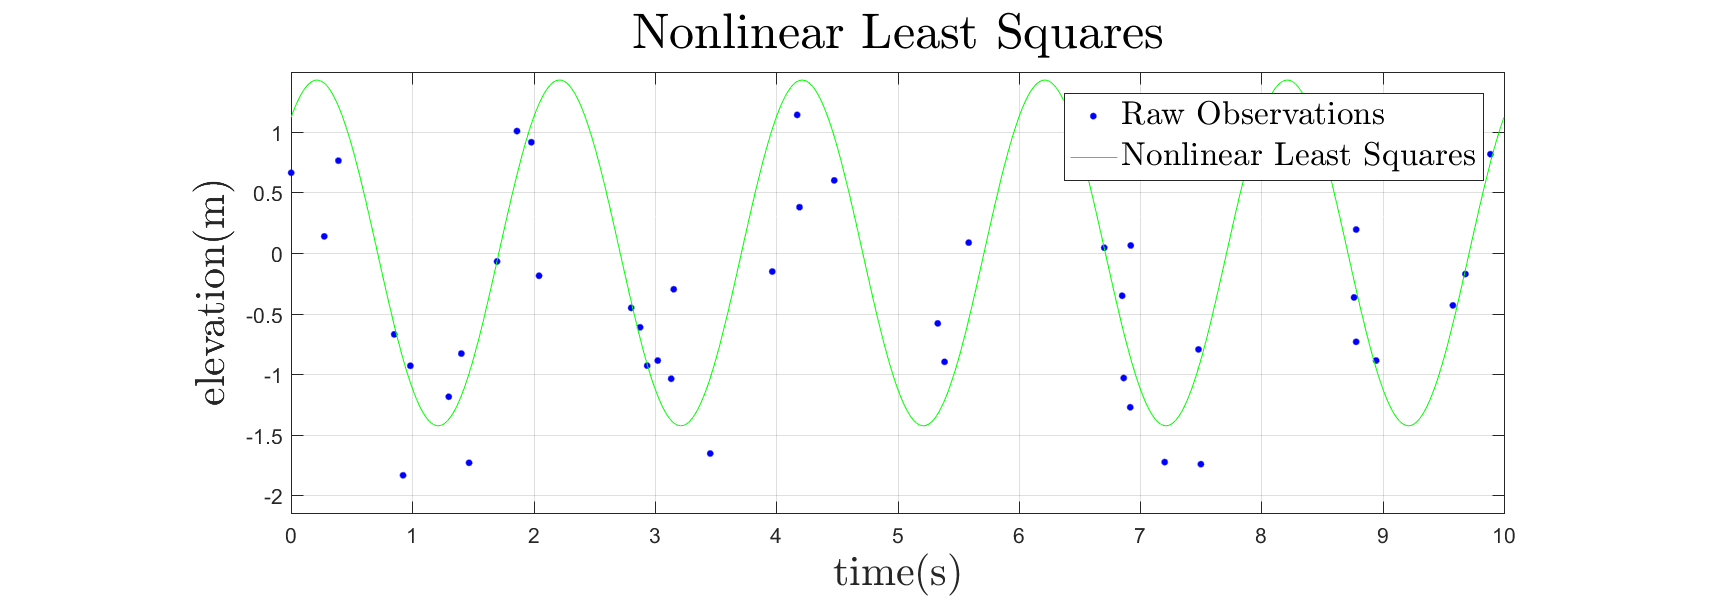
\includegraphics[height = 2in]{nonlinearresult.png}
\end{figure}

Note: The previous example could have been calculated using Weighted Least Squares (WLS)

The Observation Equation can be rewritten as:
\[
A \times \sin(\dfrac{2\pi}{T}t) + B \times \cos(\dfrac{2\pi}{T}t) = y
\]

Where $A$, $B$, $T$ are unknowns and:
\begin{align*}
	Amp &= \sqrt{A^2+B^2}\\
	\phi &= \tan^{-1}(B/A)\\
\end{align*}
\clearpage



\subsection{Example Matlab Code}
\lstinputlisting[
label      = {alg:exampleNonlinearLS},
caption    = {exampleNonlinearLS.m},
style      = Matlab-editor,
basicstyle = \mlttfamily,
firstline  = 1,
lastline   = 43,
firstnumber= 1
]{exampleNonlinearLS.m}

\lstinputlisting[
label      = {alg:exampleNonlinearLS},
caption    = {The Matlab built in function NLINFIT generates the same results},
style      = Matlab-editor,
basicstyle = \mlttfamily,
firstline  = 45,
lastline   = 49,
firstnumber= 45
]{exampleNonlinearLS.m}
